\documentclass[11pt]{article}
\usepackage[letterpaper,margin=1in]{geometry}
\usepackage[T1]{fontenc}
\usepackage{lmodern}
\usepackage{graphicx,booktabs,amsmath,amssymb,multirow,array}
\usepackage[hidelinks]{hyperref}
\usepackage{caption}
\usepackage[round,authoryear]{natbib}
\captionsetup{font=small,labelfont=bf}
\graphicspath{{figures/}}

\title{\textbf{Where Does Scoring Bias Come From?}\\
\large A Base-vs-Instruct Study of Three Scoring Biases in Small Open-Weight LLM Judges}
\author{Sricharan Samba\\
\small South Forsyth High School \\
\small \texttt{srisamba09@gmail.com}}
\date{July 2026}

\begin{document}
\maketitle

\begin{abstract}
\noindent
LLMs are widely used as automated judges, yet they show systematic \emph{scoring
biases}: their ratings shift when superficial features of the scoring task are
perturbed. \citet{li2025scoring} documented three such biases---rubric order,
score identifier, and reference-answer bias---but left open whether they
originate in pre-training or are introduced during instruction tuning. We take a
first empirical step on this question using a controlled base-vs-instruct
comparison across seven open-weight model families ($\leq$7B parameters) run on a
free GPU. Treating each family as one paired observation ($n=7$), we find that
instruction tuning \emph{reduces} bias for all three probes. The reduction is
large and robust for score-ID bias ($d_z=-1.08$, 6/7 families, bootstrap
95\% CI $[-1.54,-0.33]$) and reference-answer bias ($d_z=-1.18$, 6/7,
$[-1.27,-0.31]$), and weak and outlier-driven for rubric-order bias. We do
\emph{not} reproduce a ``content bias increases with tuning'' pattern in this
regime. Our result is consistent with scoring bias being modulated at the
instruction-tuning stage rather than fixed at pre-training, at least for small
models, and suggests instruction tuning is net-beneficial for judge robustness
here. We release a single-command pipeline that regenerates every number and
figure from one data file.
\end{abstract}

\section{Introduction}
When one language model scores another's output, we would like the score to
reflect response quality---not the wording of the rubric or the presence of an
example. Yet LLM judges are systematically sensitive to such surface features.
\citet{li2025scoring} introduced and quantified three \emph{scoring biases}:
\textbf{rubric order} (does reversing the ``1=worst\dots5=best'' scale change
scores?), \textbf{score ID} (do numeric vs.\ letter vs.\ descriptive labels
change scores?), and \textbf{reference answer} (does showing a good or poor
exemplar shift subsequent scores?). They observed these biases across five
frontier models but explicitly noted that ``the underlying causes of these
scoring biases remain to be validated.''

This paper takes one concrete step toward a cause. We ask a single, tractable
question: \emph{are these scoring biases already present in pre-trained (base)
models, or are they shaped by instruction tuning (SFT/RLHF)?} The answer matters
for mitigation---if bias is baked in at pre-training, mitigation must target data
and architecture; if it is shaped during alignment, mitigation can target the
tuning stage. Following the base-vs-instruct methodology validated by
\citet{pan2025user} and \citet{thakur2024judging} for other judge behaviours, we
compare the two variants of the same model family under identical probes.

\paragraph{Contributions.}
\begin{enumerate}\itemsep2pt
  \item A controlled base-vs-instruct comparison of all three
        \citet{li2025scoring} scoring biases across seven open-weight families
        ($\leq$7B), reproducible at zero cost.
  \item The finding that instruction tuning \emph{reduces} scoring bias in this
        regime---robustly for score-ID and reference-answer bias---rather than
        introducing it.
  \item A fully reproducible pipeline: every table and figure is regenerated by
        one script from one data file, with no manual steps.
\end{enumerate}

\paragraph{Scope.} This is a deliberately narrow, exploratory study. Our
inferential unit is the model \emph{family} ($n=7$), all models are
$\leq$7B, and only English prompts are used. We state these limits plainly
(\S\ref{sec:limits}) and frame the result as directional evidence, not a
definitive causal claim.

\section{Related Work}
\paragraph{Bias in LLM judges.} \citet{wang2023large} showed GPT-4 flips its
preferred answer 46.3\% of the time when response order is swapped;
\citet{zheng2023judging} systematised LLM-as-a-judge evaluation and noted length
and position biases; \citet{ye2024justice} catalogued twelve bias types; and
\citet{chen2024humans} found humans and LLMs share susceptibility to irrelevant
factors. \citet{shi2024position} give a systematic account of position bias, and
\citet{gu2024survey} survey the area. \citet{park2024offsetbias} mitigate bias by
tuning on debiased data.

\paragraph{Scoring bias and its causes.} \citet{li2025scoring} introduced the
three scoring biases we study and called for root-cause analysis.
\citet{thakur2024judging} observed that base and instruct Llama-2 differ as
judges, and \citet{pan2025user} used a base-vs-instruct design to show that
instruction tuning \emph{introduces} a user-deference bias absent in base models.
Our work applies the same design to \citet{li2025scoring}'s scoring biases, and
finds the opposite sign for these particular biases: tuning reduces, rather than
introduces, them.

\section{Method}
\paragraph{Models.} We use seven open-weight families for which both a
pre-trained (base) and an instruction-tuned checkpoint are publicly available:
Qwen2.5-0.5B/1.5B/7B \citep{qwen25}, Llama-3.2-1B/3B \citep{llama3},
Gemma-2-2B \citep{gemma2}, and StableLM-2-1.6B \citep{stablelm2}. This spans
0.5--7B parameters and two alignment recipes (RLHF for six families, SFT for
StableLM-2). All models are run with greedy decoding (temperature 0) on a free
Kaggle T4 GPU.

\paragraph{Probes.} We use the three perturbation probes of
\citet{li2025scoring}. \textbf{Rubric order}: normal (1=worst\dots5=best) vs.\
reversed. \textbf{Score ID}: numeric (1--5) vs.\ letter (A--E) vs.\ descriptive
(Poor--Excellent). \textbf{Reference answer}: no exemplar vs.\ a good exemplar
vs.\ a poor exemplar shown before scoring. Each model scores the same set of
instruction--response items under each variant.

\paragraph{Bias metric.} Following \citet{li2025scoring}, we summarise each
model$\times$probe by $\Delta$, the maximum spread in mean score across that
probe's variants: $\Delta = \max_v \bar{s}_v - \min_v \bar{s}_v$. Larger $\Delta$
means the model's scores move more when only the surface feature changes, i.e.\
more bias. $\Delta$ is bounded in $[0,4]$ on a 1--5 scale.

\paragraph{Unit of analysis and inference.}
The data of record retains, for each model and probe variant, the \emph{mean}
score across items---not the individual item scores.\footnote{The scores were
transcribed from the run logs of the original experiment; per-item scores were
not preserved. Consequently item-level quantities used elsewhere in the
literature---flip rate, per-item discrimination, and domain breakdowns---are not
computable here, and we do not report them.} We therefore analyse at the level of
the model \emph{family}: each family contributes one base $\Delta$ and one
instruct $\Delta$ per probe, giving $n=7$ paired observations. For each probe we
report the paired mean change (instruct $-$ base), the standardized paired effect
size $d_z$, a percentile bootstrap 95\% CI of the mean change ($10^4$ resamples,
seed 42), the two-sided exact Wilcoxon signed-rank test, and the number of
families in which bias decreased.

\section{Results}
\begin{table}[t]
\centering\small
\caption{Effect of instruction tuning on each scoring bias, across $n=7$
families. $\Delta$ is the max inter-variant score spread (lower = less biased).
\textbf{Bold} change = bootstrap 95\% CI excludes zero.}
\label{tab:summary}
% AUTO-GENERATED by repro/analyze.py -- do not edit by hand.
\begin{tabular}{lccccc}
\toprule
\textbf{Probe} & \textbf{Base} & \textbf{Instruct} & \textbf{Change} & \textbf{$d_z$} & \textbf{95\% CI} \\
 & mean $\Delta$ & mean $\Delta$ & (\%) & & (bootstrap) \\
\midrule
Rubric order & 0.69 & 0.29 & {-0.40 (-58\%)} & -0.38 & [-1.21, +0.13] \\
Score ID & 2.41 & 1.44 & \textbf{-0.97 (-40\%)} & -1.08 & [-1.54, -0.33] \\
Reference answer & 2.76 & 1.93 & \textbf{-0.83 (-30\%)} & -1.18 & [-1.27, -0.31] \\
\bottomrule
\end{tabular}

\end{table}

\begin{figure}[t]
\centering
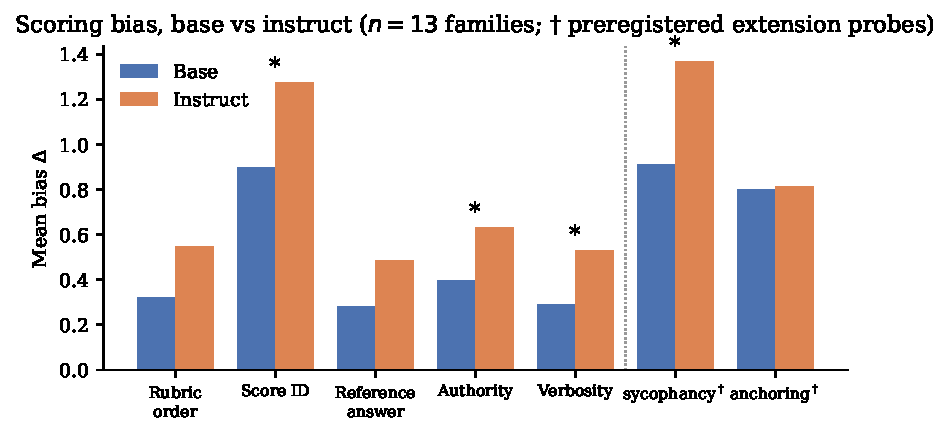
\includegraphics[width=0.72\linewidth]{fig1_base_vs_instruct.pdf}
\caption{Mean bias before and after instruction tuning. Score-ID and
reference-answer bias fall substantially; rubric-order bias is small in both.
$*$ marks a bootstrap 95\% CI on the change that excludes zero.}
\label{fig:main}
\end{figure}

\paragraph{Instruction tuning reduces all three biases.}
Table~\ref{tab:summary} and Figure~\ref{fig:main} show the headline result. Mean
bias falls from base to instruct for every probe. For \textbf{score-ID} bias the
drop is $-0.97$ points ($-40\%$; $d_z=-1.08$; 6/7 families; bootstrap CI
$[-1.54,-0.33]$), and for \textbf{reference-answer} bias it is $-0.83$ points
($-30\%$; $d_z=-1.18$; 6/7; $[-1.27,-0.31]$). Both CIs exclude zero and the exact
Wilcoxon test attains its minimum two-sided $p=0.047$ at $n=7$. \textbf{Rubric-order}
bias also decreases on average ($-0.40$), but the effect is small, not robust
(CI $[-1.21,0.13]$ includes zero, 3/7 families), and is dominated by a single
family (Llama-3.2-3B, base $\Delta=3.5$ vs.\ a median base $\Delta$ of only
$0.1$): most small base models simply are not sensitive to scale reversal.

\begin{figure}[t]
\centering
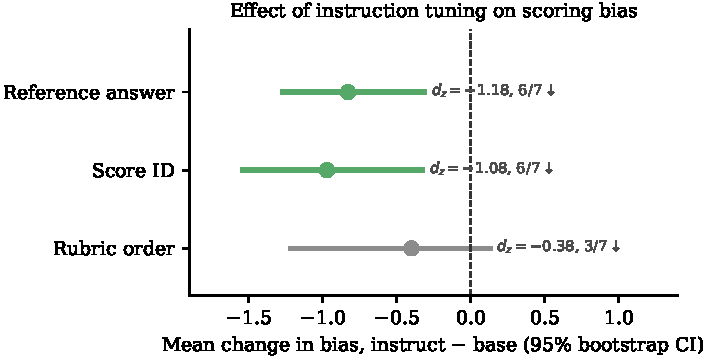
\includegraphics[width=0.66\linewidth]{fig3_forest.pdf}
\caption{Paired change in bias (instruct $-$ base) with 95\% bootstrap CIs. Green
(CI excludes zero) marks robust reductions; grey marks the inconclusive
rubric-order effect.}
\label{fig:forest}
\end{figure}

\paragraph{The reduction is consistent across families.}
Figure~\ref{fig:family} shows every family individually. For score-ID and
reference-answer bias the instruct checkpoint is less biased than its base in six
of seven families---the lone exception for both is Llama-3.2-1B, the smallest
Llama model. The consistency of direction, more than the borderline $p$-value, is
what supports the finding: with $n=7$ and three probes, we do not claim
significance survives a multiple-comparison correction, and we treat the effect
sizes and per-family agreement as the primary evidence.

\begin{table}[t]
\centering\footnotesize
\caption{Per-family bias $\Delta$ before/after instruction tuning. B = parameters
(billions); Train = alignment recipe of the instruct checkpoint.}
\label{tab:family}
\setlength{\tabcolsep}{4pt}
% AUTO-GENERATED by repro/analyze.py -- do not edit by hand.
\begin{tabular}{lcccccccc}
\toprule
\multirow{2}{*}{\textbf{Family}} & \multirow{2}{*}{\textbf{B}} & \multirow{2}{*}{\textbf{Train}} & \multicolumn{2}{c}{\textbf{Rubric order}} & \multicolumn{2}{c}{\textbf{Score ID}} & \multicolumn{2}{c}{\textbf{Reference answer}} \\
 & & & base & inst & base & inst & base & inst \\
\midrule
Qwen2.5-0.5B & 0.5 & RLHF & 0.1 & 0.2 & 1.3 & 0.4 & 2.6 & 1.2 \\
Qwen2.5-1.5B & 1.5 & RLHF & 0.1 & 0.4 & 3.1 & 1.8 & 2.6 & 1.8 \\
Llama-3.2-1B & 1 & RLHF & 0.0 & 0.2 & 1.3 & 2.0 & 2.2 & 2.6 \\
Llama-3.2-3B & 3 & RLHF & 3.5 & 0.8 & 3.7 & 2.4 & 3.1 & 2.5 \\
Gemma-2-2B & 2 & RLHF & 0.1 & 0.1 & 2.1 & 0.6 & 2.6 & 1.1 \\
StableLM-2-1.6B & 1.6 & SFT & 0.4 & 0.3 & 2.9 & 2.5 & 3.8 & 3.4 \\
Qwen2.5-7B & 7 & RLHF & 0.6 & 0.0 & 2.5 & 0.4 & 2.4 & 0.9 \\
\bottomrule
\end{tabular}

\end{table}

\begin{figure*}[t]
\centering
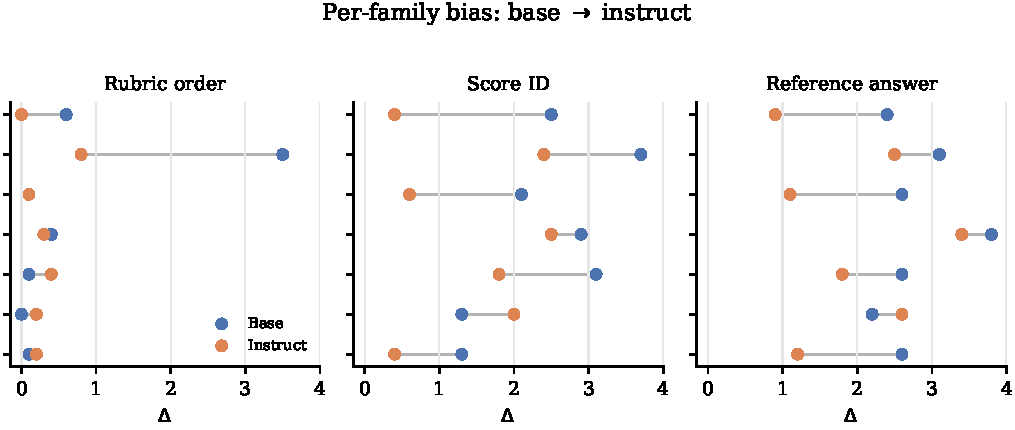
\includegraphics[width=0.92\linewidth]{fig2_family_dumbbell.pdf}
\caption{Per-family bias, base ($\bullet$, blue) $\rightarrow$ instruct
($\bullet$, orange), sorted by size. Leftward movement = bias reduced by
instruction tuning. Score-ID and reference-answer panels move left in 6/7
families each.}
\label{fig:family}
\end{figure*}

\section{Discussion}
\paragraph{Interpretation.} Base models can be strikingly biased: several assign
sharply different scores under a mere relabelling (score ID) or after seeing an
unrelated exemplar (reference answer). Instruction tuning consistently damps both.
The most parsimonious reading is that these two biases are not immutable
properties of the pre-trained network but are substantially \emph{shaped by the
instruction-tuning stage}---the same stage at which the model learns to follow the
scoring instruction in the first place. This directly addresses the open question
of \citet{li2025scoring} for small models: the cause is, at least in part,
downstream of pre-training, so mitigation targeting the tuning stage is plausible.

\paragraph{Relation to prior sign of the effect.} \citet{pan2025user} found
instruction tuning \emph{adds} a bias (user deference). We find it \emph{removes}
scoring biases. These are compatible: instruction tuning teaches a model to parse
and follow the scoring task more faithfully---helping with format-driven biases
like score ID---while separately making it more deferential to a conversational
user. Which sign dominates is bias-specific, so ``instruction tuning increases
bias'' should not be assumed as a general rule.

\paragraph{A note on mechanism.} A natural conjecture is that instruction tuning
improves how reliably the model maps a rubric label to a score, reducing
format-driven noise. We deliberately do \emph{not} present internal (e.g.\
attention-based) evidence for any mechanism: our data do not support such a claim,
and we leave mechanistic analysis to future work with instrumented model runs.

\section{Limitations}\label{sec:limits}
\begin{enumerate}\itemsep2pt
  \item \textbf{Aggregate data.} Only per-variant mean scores were retained, so
        all inference is at the family level ($n=7$). Item-level metrics (flip
        rate, discrimination, domain effects) cannot be computed and are not
        reported.
  \item \textbf{Small $n$ and low power.} With seven families the exact Wilcoxon
        test cannot fall below $p=0.047$, and a multiplicity correction across
        three probes would render it non-significant. We rely on effect sizes,
        bootstrap CIs, and directional consistency, and flag the rubric-order
        result as inconclusive.
  \item \textbf{Scale.} All models are $\leq$7B. Larger models---especially
        strong RLHF chat models---may behave differently; our data cannot speak
        to them, and we make no claim that the reduction persists at scale.
  \item \textbf{Single recipe per family, English only, greedy decoding.} We
        cannot separate SFT from RLHF contributions, generalise beyond English,
        or estimate within-model variance (temperature 0 makes repeats
        deterministic).
\end{enumerate}

\section{Conclusion}
Across seven small open-weight families, instruction tuning \emph{reduces} the
scoring biases of \citet{li2025scoring}, robustly so for score-ID and
reference-answer bias. This is directional evidence that these biases are shaped
during instruction tuning rather than fixed at pre-training, and that, for small
judges, tuning improves robustness rather than harming it. The claim is modest by
construction: it rests on seven families of aggregate data. We hope the
zero-cost, fully reproducible design lowers the barrier to the larger,
item-level, larger-scale replication needed to settle the question.

\section*{Reproducibility}
Every statistic and figure in this paper is produced by
\texttt{repro/analyze.py} and \texttt{repro/make\_figures.py} from the single
data file \texttt{t4fam\_results.json} (seed 42). No synthetic or simulated data
is used.

\section*{Ethics Statement}
No human subjects were involved. All models are publicly available open-weight
checkpoints used under their respective licenses. The experiment runs at zero
monetary cost on a free GPU tier.

\bibliographystyle{plainnat}
\bibliography{honest}

\end{document}
